\documentclass[11pt]{article}

% set these commands
\newcommand{\course}{CSCI 534}
\newcommand{\proj}{Homework 05}
\newcommand{\dueDate}{3-25-2021}
\newcommand{\instructor}{David L. Millman}

\usepackage{../macros}

\begin{document}

\coverpage{05}

\newpage
\section*{Problem 1}

In Homework 1, we considered a plane-sweep algorithm for determining whether
there is any intersection among a collection of $n$ circles in the plane. Here
we consider a variant of this problem. The input consists of a collection of $n$
closed circular disks, all having the same radius. (Via scaling, we may assume
that they are all unit disks.) Let $C = \{c_1, \ldots , c_n\}$ denote the center
points of these disks, and let $\{D_1, \ldots, D_n\}$ denote the actual disks.
Thus, $D_i$ consists of the points that lie within unit distance of $c_i$. Let
$U = D_1 \cup \ldots \cup D_n$ denote the union of these disks. The boundary of
$U$ may generally consist of multiple parts, each of which consists of a cycle
of circular arcs connected by vertices. (In Fig. 4 the boundary consists of
three cycles. The vertices are shown as white dots).

\begin{figure}[h]
    \centering
    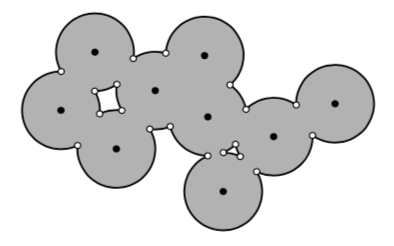
\includegraphics[width=0.4\textwidth]{union-of-disks}
    \caption{Problem 4: Union of disks}
\end{figure}


\begin{enumerate}

    \item Present an algorithm that reports all the vertices on the boundary of
        $U$. (Note that circle intersection points in the interior of the union
        are explicitly excluded.) Your algorithm should run in time $O(n \log
        n)$.  The order in which the vertices are output is arbitrary. (Hint:
        Don't try to modify the algorithm from Homework 2. A different approach
        is needed.... think giraffes)

    \item Prove that the number of vertices reported by your algorithm is
        $O(n)$.

\end{enumerate}

\answer
\begin{enumerate}
    \item The pseudocode is given in Algorithm \ref{alg:boundaryvertices}.
    But because of the page break, let's analyze run time here.
    Line 1 takes $O(1)$ time and computing the Voronoi diagram of $n$ sites on line 2 takes $O(n \log n)$ time.
    Each iteration of the for loop takes $O(1)$ time and there are $O(n)$ iterations of the for loop since the Voronoi diagram is a planar graph with $n$ faces $\implies$ the number of edges is $O(n)$.
    Thus the run time is dominated by the $O(n \log n)$ term.

    Now let's talk about correctness.
    The correctness of the algorithm is proven by the following two lemmas.
    First, boundary vertices must be on a Voronoi edge.
    Suppose we have a boundary vertex, it must be distance 1 between two different sites.
    This is exactly the property that edges of Voronoi diagrams possess so the vertex lies on a Voronoi edge.
    Second, a point on an Voronoi edge is a vertex iff the distance to the site on the left face is 1 (Voronoi properties imply the distance to the site on the right is also 1).
    Going to the left, suppose we have a point on the edge that is a boundary vertex.
    Since the point is on a Voronoi edge, it is equidistant to its two sites.
    Further, since the point is a boundary vertex it is distance 1 to the sites.
    Now going to the right, suppose we have a point on a Voronoi edge that is distance 1 to site on its left face.
    Since the point is on the edge, it is equidistant between the two sites and distance 1 implies that the point lies on a circle border.
    Now the question is, does the point lie on the boundary of the union?
    It does!
    For since the point is on a Voronoi edge its closest points (which are distance 1) must be the sites of the adjacent faces.
    Thus any other points are strictly further away than distance 1 and the point lies on the boundary of the circle.

    \begin{algorithm}
    \caption{Compute vertices}
    \label{alg:boundaryvertices}
    \begin{algorithmic}[1]
    \Function{Boundary Vertices}{$C$, $D$}
        \State P $\gets$ empty list
        \State Compute the Voronoi diagram using the circle centers as sites
        \For{each edge $e$ in the Voronoi diagram}
            \State R $\gets$ circle of radius 1 centered at either site closest to $e$
            \If{edge $e$ intersects circle R}
                \State add intersection point(s) to P
            \EndIf
        \EndFor
        \State \Return P
    \EndFunction
    \end{algorithmic}
    \end{algorithm}

    \item Now we need to show that the number of vertices reported from the algorithm is $O(n)$.
    This falls out nicely from our algorithm.
    We know the Voronoi diagram to have $n$ sites which means there are $O(n)$ edges.
    Each edge can produce a maximum of 2 points on the boundary (since it is a straight line segment intersecting a circle) so the number of points produced is $2*O(n) = O(n)$ as desired.
\end{enumerate}

\newpage
\section*{Problem 2}

Suppose we are given a subdivision of the plane into $n$ convex regions. We
suspect that this subdivision is a Voronoi diagram, but we do not know the
sites. Develop an algorithm that finds a set of $n$ point sites whose Voronoi
diagram is exactly the given subdivision, if such a set exists. \\\\

\answer
So we are given a subdivision of the plane into convex regions and we wish to report a set of $n$ sites whose Voronoi diagram is the subdivision (if it possible).
Let's consider two trivial cases before giving an algorithm.
If $n=1$, then any point works and if $n=2$ we can just take any point not on the edge of the subdivision and its reflection.
From here on out, we will assume $n > 2$.
For general position, we will assume that no vertex in the subdivision has degree higher than 3.

Label the subdivsion $D$.
Suppose for some face in $D$, we have a single point $p$ that must be the site of the face (if $D$ is a Voronoi diagram).
Assume that the faces of $D$ are labeled $1, 2, \ldots, n$.
We will prove that we can compute that point $p$ later in the problem.

Here is a quick prose description of the algoritm.
We take $D$ to be a DCEL, $p$ is the site we know must exist, and $k$ is the label for the face that $p$ belongs to.
We are going to start at $p$ and reflect it across each edge of the face $k$.
If $p$ is a site in a voronio diagram, its reflection across an edge must also be a site.
We record every reflected point in an array and add faces to a processing queue as we come across them (note each face can only be added once).
If we ever find that a newly reflected point conflicts with a point already found in that face, we know that the subdivision is not a voronoi diagram.
We now present the algorithm in pseudocode.

\begin{algorithm}
\caption{Computing the Voronoi Sites}
\label{alg:voronoisites}
    \begin{algorithmic}[1]
    \Function{VoronoiSites}{$D$, $p = (p_x, p_y)$, $k$}
        \State S $\gets [$null, $\ldots, $ null$]$ // empty array of size $n$
        \State S[$k$] $\gets p$
        \State queue $\gets [ k ]$  // a queue for face labels
        \While{queue is not empty}
            \State $i \gets$ pop the queue
            \For{every edge $e$ of face i}
                \State $j \gets $ label of the face across $e$
                \State $q \gets $ reflection of the point S[$i$] across $e$
                \If{S[$j$] $=$ null}
                    \State S[$j$] $\gets q$
                    \State add $j$ to the queue
                \Else{ {\bf if} S[$j$] $\neq q$}
                    \State \Return NOT VORONOI
                \EndIf
            \EndFor
        \EndWhile
        \State \Return S
    \EndFunction
    \end{algorithmic}
\end{algorithm}

Let's discuss run time.
As noted in the prose description, each face can only be added to the processing queue once.
This is because once a face is in the queue, it's value in S is no longer null.
Thus the while loop runs $n$ times: once for each face.
As a gross upper bound for the for loop, it can run at most $E$ times where $E$ is the number of edges in the DCEL.
Since a DCEL represents a planar graph, $E = O(n)$ so our algorithm runs in $N * O(n) = O(n^2)$ time.

And now for correctness!
We again suppose that we have a point $p$ in some face $f$ that must be a site if the subdivision is a Voronoi diagram.
Our algorithm just runs through the edges and reflects sites.
If the algorithm terminates and there were no conflicts, then we have a set of sites that will produce a Voronoi diagram that is the subdivision.
However, if a conflict ocurrs, then the edge that was reflected across was not a perpindicular bisector for the sites of the cells and the subdivision is not a Voronoi diagram.

We must now answer the question: how do we find $p$?
First we introduce a change in perspective.
Consider a vertex of the subdivsion.
By general position this is of degree three or less.
Further, the vertex must be of degree three for a degree two vertex would result in a non-convex subdivision.
Take the vertex to be our 0 and then consider the outgoing edges to be polar rays defined by an angle in $[0, 2 \pi)$.
Figure \ref{fig:solvingphi} (A) gives an example.
For a point to be a site, we must be able to reflect its ray ``around'' a vertex and end up at the same point.
Figure \ref{fig:solvingphi} (B) shows us starting with an angle $\phi$ and reflecting around the vertex to end up at $\phi'''$.
Reflect rays is quite easy in polar, just add twice the difference!
\begin{align*}
    \phi ' &= \phi + 2(\theta _1 - \phi) = 2 \theta _1 - \phi \\
    \phi '' &= \phi' + 2(\theta _2 - \phi ') = 2 \theta _2 - \phi' \\
    \phi ''' &= \phi'' + 2(\theta _3 - \phi '') = 2 \theta _3 - \phi''
\end{align*}
For $\phi$ to be the ray that the site lies on, we must have $\phi + 2 \pi = \phi'''$.
Then substituting in our equations above, we find that $\phi = \theta _3 - \theta _2 + \theta _1 - \pi$.
This gives us a fixed ray that the site must lie on!

\begin{figure}[h]
    \centering
    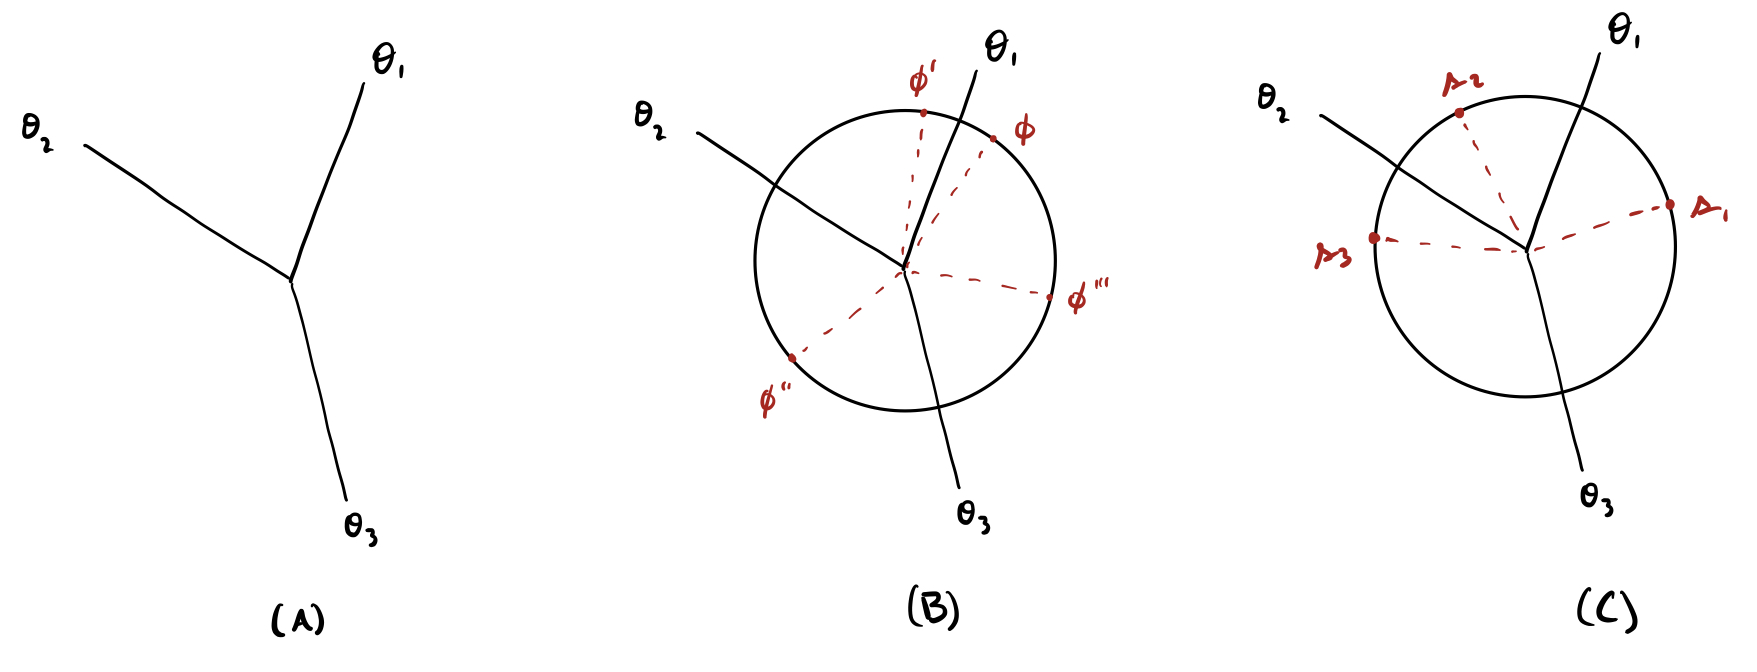
\includegraphics[width=0.9\textwidth]{solvingphi}
    \caption{Solving for $\phi$}
    \label{fig:solvingphi}
\end{figure}

\newpage
We then enter one of two cases.
Case 1: every edge in the subdivision extends off to infinity.
In this case, we can select any point on the ray as our initial site.
This is depicted in the left of Figure \ref{fig:site}.
Case 2: there exists some finite edge.
In this case, there is more work to be done.
Let $e$ be a finite edge.
Then we can solve for the ray originating on either end of the edge and compute where they intersect.
This is the unique point in the face that must be the site.

\begin{figure}[h]
    \centering
    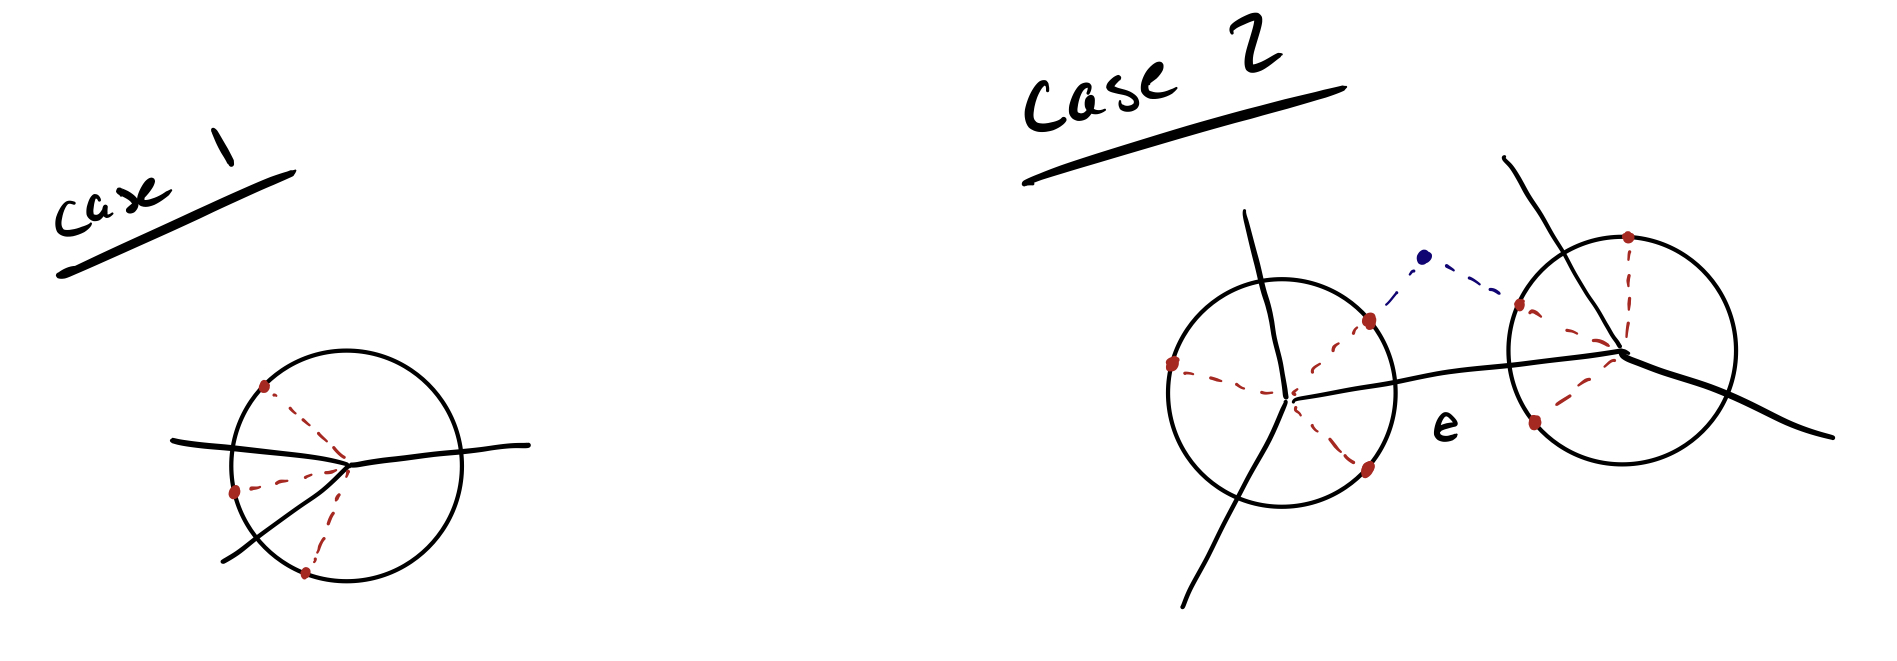
\includegraphics[width=0.6\textwidth]{site}
    \caption{Computing the site}
    \label{fig:site}
\end{figure}

Thus we can always compute our initial point $p$ and run the algorithm.
Note that this takes $O(1)$ time, so it does not affect our run time analysis.

\end{document}
